\newpage
\clearpage

% 1. Ejercicio 12:
\section{Ejercicio 12}

% 1.1. Enunciado:
\subsection{Enunciado}
\noindent Dadas las rectas $r1)
	\begin{cases}
		3x - 2y + z = 5 \\
		2x + y - z = 5
	\end{cases}$
y $r2) \ \dfrac{x - 1}{2} = \dfrac{y - 3}{10} = \dfrac{z + 2}{14}$

\begin{enumerate}
	\item Verifiquen que son paralelas y no coincidentes.
	\item Hallen la ecuación del plano que determinan.
	\item Hallen las ecuaciones de todos los planos paralelos a ambas rectas que se encuentran a 10 unidades del origen de coordenadas.
\end{enumerate}


% 1.2. Solución analítica:
\newpage
\subsection{Solución analítica}

% Valores iniciales:
\subsubsection*{Valores iniciales:}

\begin{multicols}{2}
	$r1)
		\begin{cases}
			3x - 2y + z - 5 = 0 \hspace{1cm} (\alpha) \\
			2x + y - z - 5 = 0  \hfill (\beta)
		\end{cases}$

	$r2) \ \dfrac{x - 1}{2} = \dfrac{y - 3}{10} = \dfrac{z + 2}{14}$
\end{multicols}

\noindent \textbf{A continuación buscamos los vectores $\vec{u_1} \parallel r1$ y $\vec{u_2} \parallel r2$:}

\noindent Dados los vectores normales a los planos que determinan $r1)$:

\begin{center}
	$\vec{n_{\alpha}} = (3, -2, 1) \hspace*{1cm} \vec{n_{\beta}} = (2, 1, -1)$
\end{center}
\vspace{0.5cm}
\noindent Hallamos el vector director de
$r1): \ \vec{u_1} / \vec{u_1} \perp \vec{n_{\alpha}} \land \vec{u_1} \perp \vec{n_{\beta}}$:
\begin{align*}
	\vec{u_1}              & = \vec{n_{\alpha}} \times \vec{n_{\beta}}          \\
	\vec{u_1}              & = \begin{vmatrix}
		                           i & j  & k  \\
		                           3 & -2 & 1  \\
		                           2 & 1  & -1
	                           \end{vmatrix}                                   \\
	\vec{u_1}              & = \vec{i}(2 - 1) - \vec{j}(-3 -2) + \vec{k}(3 + 4) \\
	\vec{u_1}              & = \vec{i}(1) - \vec{j}(-5) + \vec{k}(7)            \\
	\vec{u_1}              & = \vec{i} + 5\vec{j} + 7\vec{k}                    \\
	\therefore \ \vec{u_1} & = \boxed{(1, 5, 7)}
\end{align*}

\noindent Hallamos $\vec{u_2}$ de $r2$ igualando cada expresión a un $\lambda$ dado, con lo que obtenemos la siguiente ecuación paramétrica:

\begin{center}
	$r2)
		\begin{cases}
			x = 1 + 2\lambda  \\
			y = 3 + 10\lambda \\
			z = -2 + 14\lambda
		\end{cases}$ \\
	\vspace{0.3cm}
	\noindent $\therefore \ \boxed{\vec{u_2} = (2, 10, 14)}$  \\
	\vspace{0.3cm}
	Obtenemos también el punto $P_0(1,3,-2)$
\end{center}



% 1.2.1. Verificación de paralelismo:
\newpage
\subsubsection{Verificación de paralelismo y rectas no coincidentes:}
\begin{center}
	$\vec{u_1} \parallel \vec{u_2} \iff \exists k \in \mathbb{R} \ / \ \vec{u_1} = k\vec{u_2}$ \\
	\vspace{0.3cm}
	$\vec{u_1} = (1, 5, 7) \hspace{1cm} \vec{u_2} = (2, 10, 14)$
\end{center}

\begin{multicols}{2}
	\begin{align*}
		\vec{u_1} & \overset{?}{=} k\vec{u_2}     \\
		(1, 5, 7) & \overset{?}{=} k(2, 10, 14)   \\
		(1, 5, 7) & \overset{?}{=} (2k, 10k, 14k)
	\end{align*}
	\columnbreak
	\begin{align*}
		1 = 2k  & \implies k = \dfrac{1}{2} \\
		5 = 10k & \implies k = \dfrac{1}{2} \\
		7 = 14k & \implies k = \dfrac{1}{2}
	\end{align*}
\end{multicols}
\begin{center}
	$\implies \vec{u_1} = \frac{1}{2}\vec{u_2} \hspace{1cm} \implies \vec{u_1} \parallel \vec{u_2} \hspace{1cm} \therefore \ \fcolorbox{black}{yellow}{$r1 \ \parallel \ r2$}$
\end{center}

\vspace{1cm}
\noindent \textbf{Son rectas coincidentes?}

\noindent Si $P_0 \in r2 \land P_0 \in r1 \implies P_0$ debe satisfacer todas las ecuaciones de $r1$:

\noindent Reemplazamos $P_0$ en la ecuación $(\alpha)$ de $r1$:
\begin{align*}
	3x - 2y + z - 5        & = 0    \\
	3(1) - 2(3) + (-2) - 5 & = 0    \\
	3 - 6 -2 - 5           & = 0    \\
	3 - 13                 & = 0    \\
	-10                    & \neq 0
\end{align*}

\noindent Pero $P_0$ \textbf{no satisface} la ecuación una de las ecuaciones de $r1$, entonces $P_0$ no pertenece a $r1$.
\begin{center}
	$\therefore \fcolorbox{black}{yellow}{$r1 \land r2 \ \ \text{no son coincidentes}$}$
\end{center}

\vspace{1cm}
\noindent \textbf{Gráfica}:
\begin{center}
	\href{https://www.geogebra.org/3d/yqkppcut}{\includegraphics[width=13cm, scale=0.8]{TP-MATEMÁTICA-EJ12A.png}}
\end{center}



% 1.2.2. Ecuación del plano:
\newpage
\subsubsection{Ecuación del plano que determinan $r1$ y $r2$:}
\noindent  \textbf{Información inicial}:
\begin{multicols}{2}
	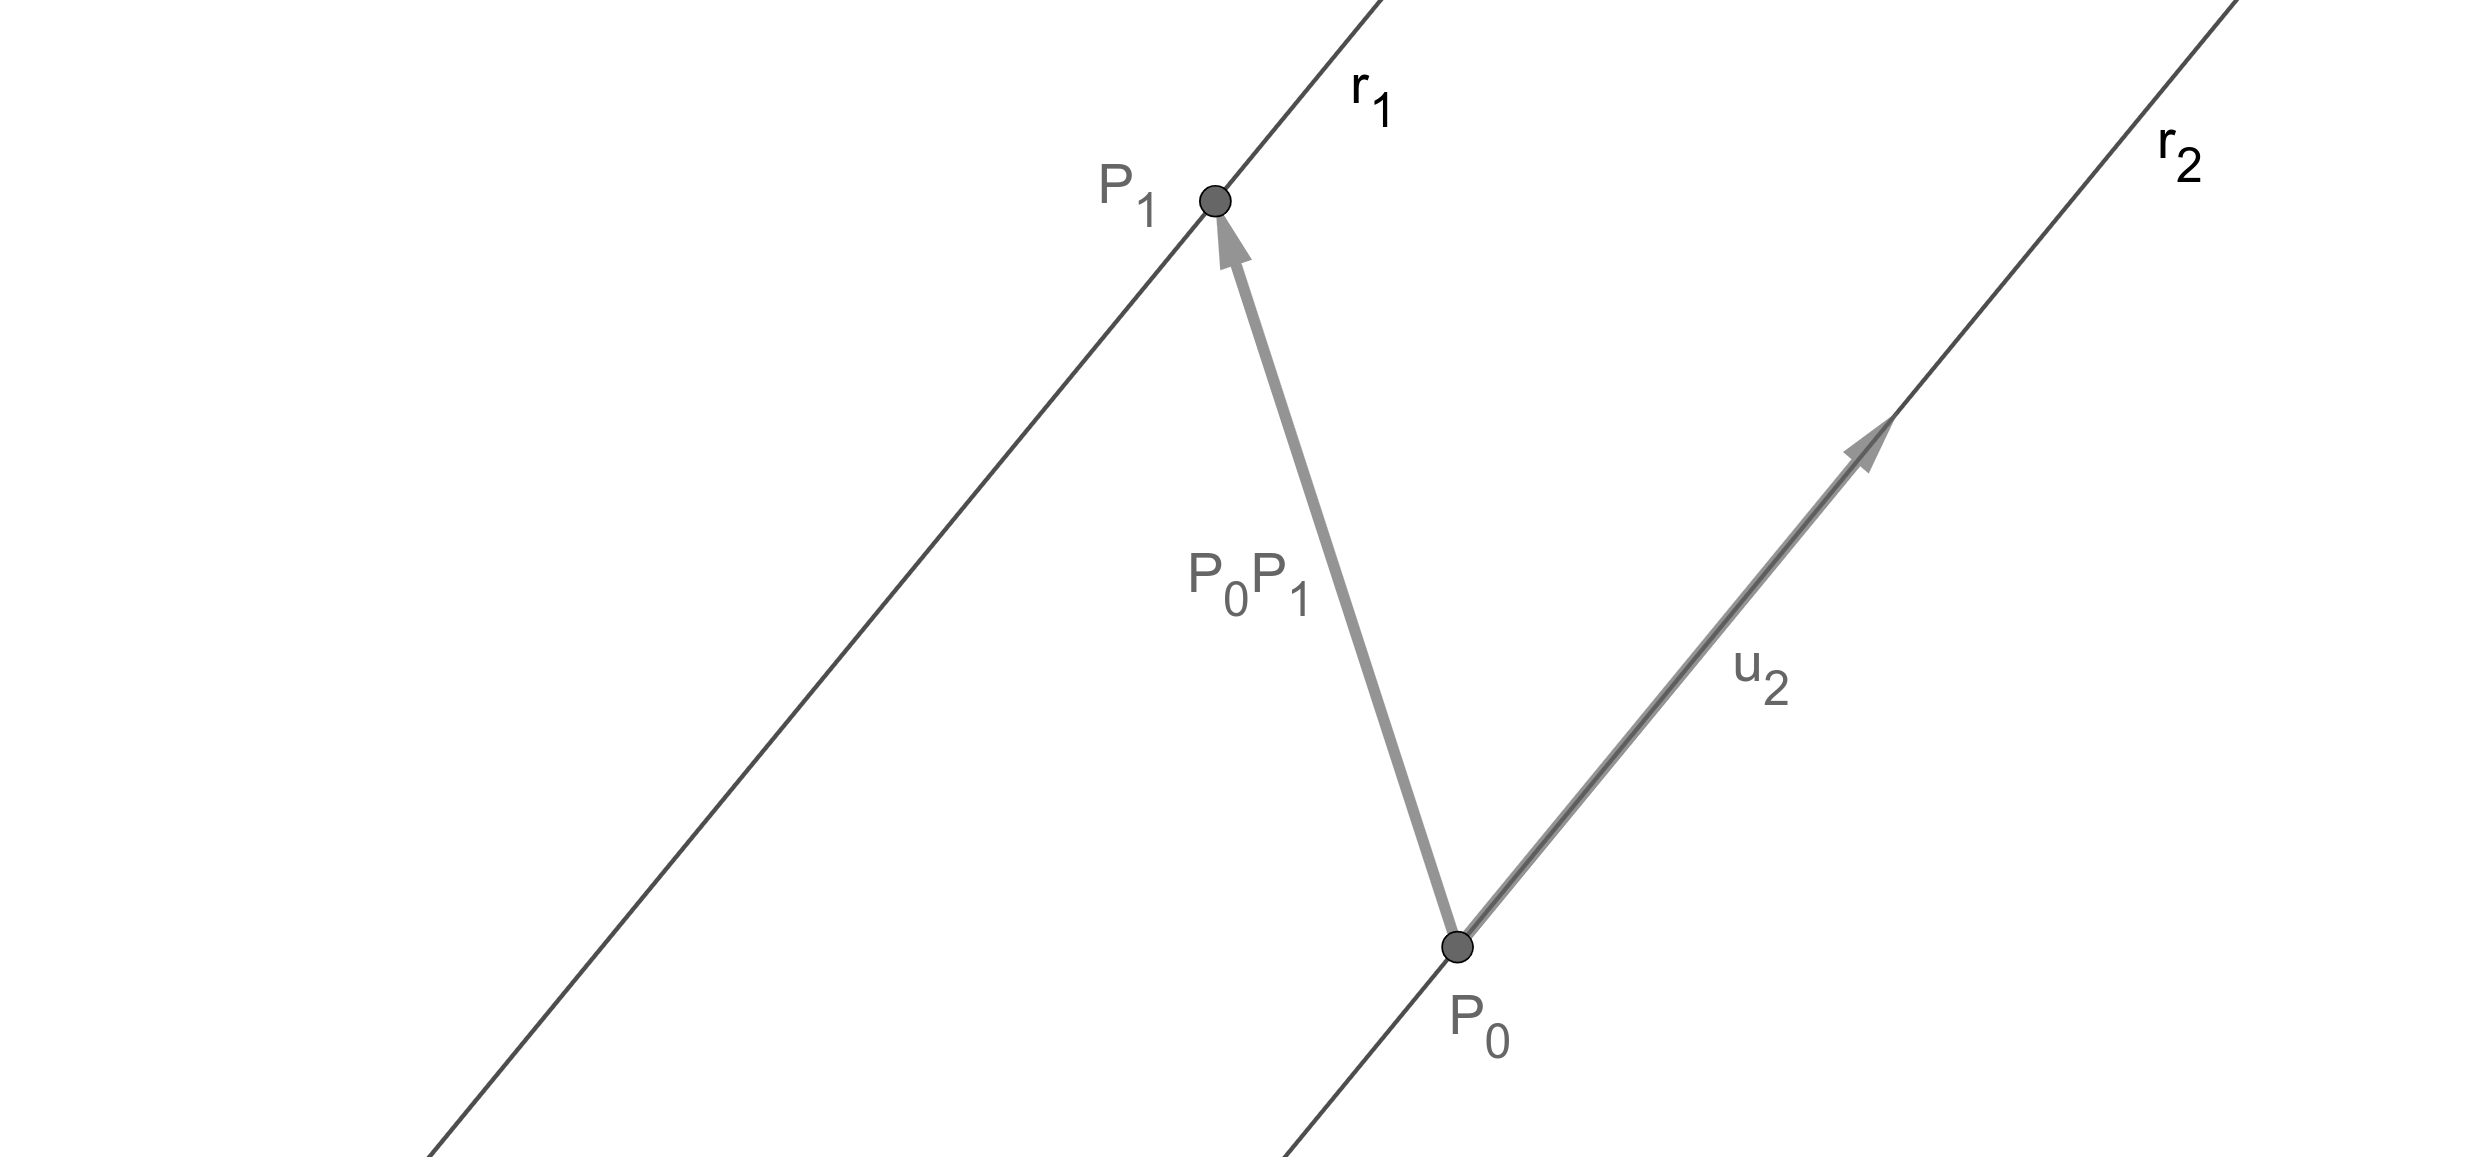
\includegraphics[width=7cm, scale=0.8]{12b1.png} \\
	$\overrightarrow{P_0P_1} \times \vec{u_2} = \vec{n}$, vector normal al plano determinado por $\overrightarrow{P_0P_1}$ y $\vec{u_2}$.
\end{multicols}

\noindent \textbf{Buscamos un punto de paso $P_1$ en $r1$}:
\begin{multicols}{2}
	\noindent Si $z=\boxed{0} \implies \begin{cases}
			3x - 2y - 5 = 0 \hspace{0.5cm} (1) \\
			2x + y - 5 = 0 \hfill (2)
		\end{cases}$

	\noindent Despejamos $y$ de $(1)$:
	\begin{align*}
		3x - 2y - 5 & = 0                                    \\
		-2y         & = -3x + 5                              \\
		y           & = \dfrac{-(3x - 5)}{-2}                \\
		y           & = \dfrac{3x - 5}{2} \hspace{0.5cm} (3)
	\end{align*}

	\noindent Reemplazamos $(3)$ en $(2)$ para hallar $x$:
	\begin{align*}
		2x + y - 5                                & = 0                    \\
		2x + \left( \dfrac{3x - 5}{2} \right) - 5 & = 0                    \\
		2x + \dfrac{3x}{2} - \dfrac{5}{2} -5      & =0                     \\
		\dfrac{7}{2}x - \dfrac{15}{2}             & = 0                    \\
		7x - 15                                   & = 0                    \\
		x                                         & =\boxed{\dfrac{15}{7}}
	\end{align*}

	Reemplazamos $x$ en $(3)$ para hallar $y$:
	\begin{align*}
		y & = \dfrac{3x - 5}{2}                                      \\
		y & = \dfrac{3}{2}x - \dfrac{5}{2}                           \\
		y & = \dfrac{3}{2} \left(\frac{15}{7} \right) - \dfrac{5}{2} \\
		y & = \dfrac{45}{14} - \dfrac{35}{14}                        \\
		y & = \dfrac{10}{14}                                         \\
		y & = \boxed{\dfrac{5}{7}}                                   \\
	\end{align*}

	$\therefore \ \boxed{P_1 \left (\frac{15}{7}, \frac{5}{7}, 0 \right) \in r1}$
\end{multicols}

\vspace{6cm}
%\vfill
\noindent \textbf{A partir de este punto de paso $P_1$ podemos buscar el vector $\vec{n'}$ del plano determinado por $r1$ y $r2$}:

\begin{center}
	$P_0(1, 3, -2) \hspace{1cm} P_1 \left (\frac{15}{7}, \frac{5}{7}, 0 \right)$
\end{center}

%\newpage
\noindent Armamos el vector $\overrightarrow{P_0P_1}$:
\begin{align*}
	\overrightarrow{P_0P_1} & = \left (\frac{15}{7}, \frac{5}{7}, 0 \right) - (1, 3, -2)       \\
	\overrightarrow{P_0P_1} & = \left (\frac{15}{7} - 1, \ \frac{5}{7} - 3, \ 0 - (-2) \right) \\
	\overrightarrow{P_0P_1} & = \left (\frac{8}{7}, \ -\frac{16}{7}, \ 2 \right)               \\
\end{align*}

\noindent Buscamos el vector $\vec{n'}$ con $\overrightarrow{P_0P_1}$ y $\vec{u_2}$:
\begin{align*}
	\vec{n'}              & = \overrightarrow{P_0P_1} \times \vec{u_2}                         \\
	\vec{n'}              & = \begin{vmatrix}
		                          i           & j             & k  \\
		                          \frac{8}{7} & -\frac{16}{7} & 2  \\
		                          2           & 10            & 14
	                          \end{vmatrix}                                 \\
	\vec{n'}              & = \vec{i} \left[(-\frac{16}{7})\cdot(14) - (2)\cdot(10) \right]  +
	\vec{j} \left[ (2)\cdot(2) - (\frac{8}{7})\cdot(14) \right] +
	\vec{k} \left[ (\frac{8}{7})\cdot(10) - (-\frac{16}{7})\cdot(2) \right]                    \\
	\vec{n'}              & = \vec{i} \left[-32 - 20 \right]  +
	\vec{j} \left[ 4 - 16 \right] +
	\vec{k} \left[ \frac{80}{7} + \frac{32}{7} \right]                                         \\
	\vec{n'}              & = \vec{i} (-52) + \vec{j} (- 12) + \vec{k} (16)                    \\
	\vec{n'}              & = -52\vec{i}- 12\vec{j} + 16\vec{k}                                \\
	\vec{n'}              & = -13\vec{i}- 3\vec{j} + 4\vec{k}                                  \\
	\therefore \ \vec{n'} & = \boxed{(-13, -3, 4)}
\end{align*}

\noindent Con el vector $\vec{n'}$ encontrado empezamos a armar la ecuación del plano al que llamaremos $\omega$:
\begin{center}
	$\omega) \hspace{1cm} -13x - 3y + 4z + d = 0$
\end{center}

\noindent Usamos el punto $P_0(1, 3, -2)$ para determinar el valor de $d$:
\begin{align*}
	-13x - 3y + 4z + d        & = 0          \\
	-13(1) - 3(3) + 4(-2) + d & = 0          \\
	-13 - 9 - 8 + d           & = 0          \\
	-30 + d                   & = 0          \\
	d                         & = \boxed{30}
\end{align*}

\noindent $\therefore \ \fcolorbox{black}{yellow}{$\omega) \ \ -13x - 3y + 4z + 30 = 0$}$ es la ecuación del plano determinado por las rectas $r1$ y $r2$.

\vspace{2cm}
\noindent \textbf{Gráfica}:
\begin{center}
	\href{https://www.geogebra.org/3d/n89vhber}{\includegraphics[width=15cm, scale=1]{TP-MATEMÁTICA-EJ12B.png}}
\end{center}

% 1.2.3. Ecuaciones de planos paralelos:
\newpage
\subsubsection{Ecuaciones de planos paralelos a $r1$ y $r2$ que se encuentran a 10 unidades del origen de coordenadas:}
\noindent Planos paralelos a ambas rectas serán paralelos a $\omega$. Se podría usar el mismo vector normal $\vec{n}$ y hallar los puntos de paso a unidades del origen de coordenadas.

\noindent Valores iniciales:
\begin{center}
	$\vec{n} = (-13, -3, 4)$
\end{center}

\begin{multicols}{2}
	\noindent Hallamos el módulo de $\vec{n}$:
	\begin{align*}
		\abs{\vec{n}} & = \sqrt{(-13)^2 + (-3)^2 + (4)^2} \\
		\abs{\vec{n}} & = \sqrt{169 + 9 + 16}             \\
		\abs{\vec{n}} & = \sqrt{194}
	\end{align*}
	\columnbreak \\
	\noindent Hallamos el versor de $\vec{n}$:
	\begin{align*}
		\vec{n_0} & = \dfrac{1}{\abs{\vec{n}}} \cdot \vec{n}                                             \\
		\vec{n_0} & = \dfrac{1}{\sqrt{194}} \cdot (-13, -3, 4)                                             \\
		\vec{n_0} & = \left(\dfrac{-13}{\sqrt{194}}, \dfrac{-3}{\sqrt{194}}, \dfrac{4}{\sqrt{194}} \right)
	\end{align*}
\end{multicols}

\noindent Hallamos un vector $\vec{n_1} = 10 \cdot \vec{n_0}$ que nos servirá para hallar los puntos $P_1$ y $P_2$ que equidistan del plano en direcciones opuestas en 10 unidades:
\begin{align*}
	\vec{n_1} & = 10 \cdot \vec{n_0}                                                                           \\
	\vec{n_1} & = 10 \cdot \left(\dfrac{-13}{\sqrt{194}}, \dfrac{-3}{\sqrt{194}}, \dfrac{4}{\sqrt{194}} \right) \\
	\vec{n_1} & = \left(\dfrac{-130}{\sqrt{194}}, \dfrac{-30}{\sqrt{194}}, \dfrac{40}{\sqrt{194}} \right)       \\
\end{align*}
\begin{center}
	$\therefore \ \boxed{P_1 = \left(\dfrac{-130}{\sqrt{194}}, \dfrac{-30}{\sqrt{194}}, \dfrac{40}{\sqrt{194}} \right)}
		\ \land \ P_2 = -P_1 \implies
		\boxed{P_2 = \left(\dfrac{130}{\sqrt{194}}, \dfrac{30}{\sqrt{194}}, \dfrac{-40}{\sqrt{194}} \right)}$
\end{center}

\vspace{1cm}
\noindent A continuación hallamos las ecuaciones de los planos $\omega_1$ y $\omega_2$:

\noindent Usamos $P_1$ para hallar $\omega_1$:
\begin{align*}
	-13x - 3y + 4z + d                                 & = 0                     \\
	-13 \cdot \left( \dfrac{-130}{\sqrt{194}}\right)
	- 3 \cdot \left( \dfrac{-30}{\sqrt{194}}\right)
	+ 4 \cdot \left( \dfrac{40}{\sqrt{194}}\right) + d & = 0                     \\
	\dfrac{1690}{\sqrt{194}} + \dfrac{90}{\sqrt{194}}
	+ \dfrac{160}{\sqrt{194}} + d                      & = 0                     \\
	\dfrac{1940}{\sqrt{194}} + d                       & = 0                     \\
	10\sqrt{194} + d                                   & = 0                     \\
	d                                                  & = \boxed{-10\sqrt{194}}
\end{align*}
$\implies \ \omega_1) \ -13x - 3y + 4z -10\sqrt{194} = 0$

\noindent Usamos $P_2$ para hallar $\omega_2$:
\begin{align*}
	-13x - 3y + 4z + d                                  & = 0                    \\
	-13 \cdot \left( \dfrac{130}{\sqrt{194}}\right)
	- 3 \cdot \left( \dfrac{30}{\sqrt{194}}\right)
	+ 4 \cdot \left( \dfrac{-40}{\sqrt{194}}\right) + d & = 0                    \\
	- \dfrac{1690}{\sqrt{194}} - \dfrac{90}{\sqrt{194}}
	- \dfrac{160}{\sqrt{194}} + d                       & = 0                    \\
	- \dfrac{1940}{\sqrt{194}} + d                      & = 0                    \\
	- 10\sqrt{194} + d                                  & = 0                    \\
	d                                                   & = \boxed{10\sqrt{194}}
\end{align*}
$\implies \ \omega_2) \ -13x - 3y + 4z + 10\sqrt{194} = 0$

\vspace{1cm}
\noindent $\therefore$ Las ecuaciones de los planos paralelos a $r1$ y $r2$ que se encuentran a 10 unidades del origen de coordenadas son:

\begin{center}
	$\fcolorbox{black}{yellow}{$\omega_1) \ -13x - 3y + 4z -10\sqrt{194} = 0$} \hspace*{0.5cm}$ y
	$\hspace*{0.5cm} \fcolorbox{black}{yellow}{$\omega_2) \ -13x - 3y + 4z + 10\sqrt{194} = 0$}$
\end{center}

\vspace{2cm}
\noindent \textbf{Gráfica 12-c}:
\begin{center}
	\href{https://www.geogebra.org/3d/fmkxhwqc}{\includegraphics[width=15cm, scale=1]{TP-MATEMÁTICA-EJ12C.png}}
\end{center}


% 1.3. Gráfica de la solución:
\newpage
\subsection{Gráfica de la solución}
